\section{Alpha-decay and shell-model rules}
\subsection*{(a)}
\begin{figure}[H]
	\centering
	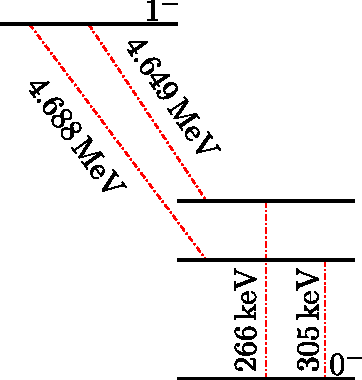
\includegraphics[width=0.75\textwidth]{figures/6b.pdf}
	\caption{Decay scheme of the alpha decay.}
\end{figure}

\subsection*{(b)}
Both are odd-odd since the ground state of the daughter has integer spin, which indicates that it is not even-odd, and since even-even have even parity in the ground state the daughter must be odd-odd. The parent state differs by two neutrons and two protons so it must also be odd-odd.

\subsection*{(c)}
The selection rules tells us that parity must be conserved. Thus we have to go from odd spin, odd parity, to even spin, even parity. However to the ground state is even spin, odd parity, which then isn't allowed.

\subsection*{(d)}
Allowed transfers, as said in (c), are from the odd spin, odd parity, to e.g. even spin, even parity. The most probable transition for an alpha is to not change spin parity between the initial and final state. Thus the most probable spin parity for the excited states is $1^-$. So both could have the same spin parity but with different configurations in the orbitals.
